\documentclass[12pt]{report}

%% Useful packages
\usepackage[a4paper,top=3cm,bottom=3cm,left=3.7cm,right=2.5cm,marginparwidth=1.75cm,headheight=22pt]{geometry}
\usepackage[hidelinks]{hyperref} %you can remove for red bounding box around links
\usepackage{amsmath}
\usepackage{cite}
\usepackage{courier}
\usepackage{listings}
\usepackage[titletoc]{appendix}
\usepackage[export]{adjustbox}
\usepackage[nottoc,notlot,notlof]{tocbibind}
\usepackage[font=small,labelfont={bf,it}, textfont=it]{caption}
\usepackage{graphicx}
\usepackage{booktabs}
\usepackage[bottom]{footmisc}
\usepackage{hyperref}
\usepackage{float}
\usepackage{setspace}
\usepackage{subfigure}
\usepackage{setspace}
\usepackage{lipsum}
\usepackage{fancyhdr} % Fancy header
\usepackage{url}
\usepackage{tabularx}
\usepackage[utf8]{inputenc}
\usepackage{mathptmx} %Times Font
\usepackage{csquotes}
\usepackage{titlesec}
\usepackage{colortbl}
\usepackage[colorinlistoftodos]{todonotes}
\setlength{\marginparwidth}{3cm} % set the width of the todo
\reversemarginpar % sets the todo in the left margin
\usepackage{enumitem}



%==== Header and Footer configure ====
% Define the plain pagestyle used by most chapters
\fancypagestyle{plain}{
\fancyhf{} % Clear header footer
\fancyhead[R]{\bf \small \textsl{\nouppercase{\leftmark}} \vspace{0.1in}}
\fancyfoot[R]{\thepage}
% Set the right side of the footer to be the page number
\renewcommand{\headrulewidth}{2pt}
}

%==== Overall Config ====
%\setlength{\parindent}{0in} % Set paragraph indent as 0
% \setlength{\fboxsep}{-0.3in}%

\titleformat{\chapter}{\centering\bfseries\large}{\chaptername~\thechapter:}{0.5em}{}
\titlespacing*{\chapter}{0pt}{0pt}{40pt}
\titleformat*{\section}{\bfseries\fontsize{12pt}{12}}
\titleformat*{\subsection}{\bfseries\itshape\fontsize{12pt}{12}}

\setlength{\fboxrule}{0.5pt} % Set the bounding box around the image as 0.5pt
\pagestyle{plain}

% \renewcommand{\chaptermark}[1]{\markboth{#1}{}}% Comment this line to use header "Chapter 1. Literature View"; otherwise header is "Literature View"

\addtocontents{toc}{\protect\vspace{0.05in}}
\addtocontents{lof}{\protect\vspace{0.05in}}
\addtocontents{lot}{\protect\vspace{0.05in}}

% Listings package settings
\lstset{
    language=Python,
    basicstyle=\scriptsize\ttfamily,
    tabsize=4,
    breaklines=true,
    breakatwhitespace=true,
    showstringspaces=false
}

\begin{document}
\fontdimen2\font=0.5em% inter word space
%==== FRONT PART====
\begin{titlepage}

\begin{figure}[h!]
\centering

\includegraphics[width=0.5\textwidth, right]{Figures/logo.png}
\caption*{}
\label{fig:entropy} 
\end{figure}

\vspace{0.5in}

\centering
\Huge{\textbf{Dynamic Difficulty adjustment aided by Reinforcement Learning Agents in Real Time Strategy games. \\Also Second Line}}\\[2.0in]

\large{\textit{\textbf{Joshua James Polanszky}}} \\[0.2in]
\large{\textit{\textbf{Supervisor: Ms Maureen Cristina}}} \\[0.8in]

\vspace{1.5in}

\normalsize{\textbf{June - 2025}}\\[0.2in]

\normalsize{\textbf{A dissertation submitted to the Institute of Information and Communication Technology in partial fulfilment of
the requirements for the degree of BSc (Hons) Multimedia in Software Development}}\\[0.2in]


\end{titlepage}
\newpage % Coverpage

%\begingroup
%\let\cleardoublepage\clearpage
\pagenumbering{roman}

%=== Authorship Statement ===
\newpage

\chapter*{\centering Authorship Statement}
\markboth{Authorship Statement}{}
\vspace{-0.2in}

\begin{spacing}{1.5}
\setlength{\parskip}{0.3in}
\setlength{\parindent}{0in}

\addcontentsline{toc}{chapter}{Authorship Statement}

This dissertation is based on the results of research carried out by myself, is my
own composition, and has not been previously presented for any other certified
or uncertified qualification.

The research was carried out under the supervision of (name of dissertation tutor
–Title, Name and surname)

\vspace{2.5cm}

\begin{center}
	\makebox[4cm]{\dotfill}  \hfill \makebox[4cm]{\dotfill}\\
	\makebox[4cm]{Date}      \hfill \makebox[4cm]{Signature}
\end{center}
\end{spacing}
\newpage
%=== END OF ABSTRACT ===

%=== Copyright Statement ===
\newpage

\chapter*{\centering Copyright Statement}
\markboth{Copyright Statement}{}
\vspace{-0.2in}

\begin{spacing}{1.5}
\setlength{\parskip}{0.3in}
\setlength{\parindent}{0in}

\addcontentsline{toc}{chapter}{Copyright Statement}

In submitting this dissertation to the MCAST Institute of Information and Com-
munication Technology, I understand that I am giving permission for it to be
made available for use in accordance with the regulations of MCAST and the
Library and Learning Resource Centre. I accept that my dissertation may be
made publicly available at MCAST’s discretion.

\vspace{2.5cm}

\begin{center}
	\makebox[4cm]{\dotfill}  \hfill \makebox[4cm]{\dotfill}\\
	\makebox[4cm]{Date}      \hfill \makebox[4cm]{Signature}
\end{center}
\end{spacing}
\newpage
%=== END OF ABSTRACT ===

%=== FRONT PART ===
%=== ACKNOWLEDGEMENT ===

%\begin{center}
\chapter*{\centering Acknowledgements}
\markboth{Acknowledgements}{}
\begin{spacing}{1.5}
\vspace{-0.2in}
\setlength{\parskip}{0.3in}
\setlength{\parindent}{0in}
%\end{center}

\addcontentsline{toc}{chapter}{Acknowledgements}

The list of people that the Student would like to thank on the completion of the dissertation. For example ‘Mr Name Surname, who supported me during my dissertation work as my tutor’.

\end{spacing}
\newpage
%=== END OF ACKNOWLEDGEMENT  ===

%=== FRONT PART ===
%=== ABSTRACT ===
\newpage

\chapter*{\centering Abstract}
\markboth{Abstract}{}
\vspace{-0.2in}

\begin{spacing}{1.5}
\setlength{\parskip}{0.3in}
\setlength{\parindent}{0in}

\addcontentsline{toc}{chapter}{Abstract}

This section should clearly state what the study is about, summarizing how it was carried out and what the results were. References are not to be included in the abstract. It should present only the essentials of the work in general. 

\par
\textbf{Keywords:} Dissertation, keywords.
\end{spacing}
\newpage
%=== END OF ABSTRACT ===



\renewcommand*\contentsname{\centering Table of Contents}
\tableofcontents

\newpage


\renewcommand{\listfigurename}{\centering List of Figures}
\listoffigures
\addcontentsline{toc}{chapter}{List of Figures}
\newpage

\renewcommand{\listtablename}{\centering List of Tables}
\listoftables 
\addcontentsline{toc}{chapter}{List of Tables}
\newpage

%=== FRONT PART ===
%=== List of Abbreviations ===
%\begin{center}
\chapter*{\centering List of Abbreviations}
\markboth{List of Abbreviations}{}

\begin{spacing}{1.5}
\setlength{\parskip}{0.3in}
%\end{center}
\addcontentsline{toc}{chapter}{List of Abbreviations}

\begin{table}[ht]
\centering
% \resizebox{0.8\textwidth}{!}{% Uncomment to set fixed width
\begin{tabular}{ll}
\textbf{NN} & Neural Network \\
\textbf{ML} & Machine Learning \\
\textbf{DL} & Deep Learning \\
\textbf{FCN} & Fully Convolutional Network \\
\textbf{CNN} & Convolutional Neural Network \\
\end{tabular}%
% }
\end{table}

\end{spacing}
\newpage
%=== END OF List of Abbreviations ===



%\endgroup

%==== MAIN PART ====

\pagenumbering{arabic}
%=== CHAPTER ONE (1) ===
%=== INTRODUCTION ===

\chapter{Introduction}
\begin{spacing}{2.0}
%\setlength{\parskip}{0.2in}

In this section, \textbf{you}, the Student, are expected to state clearly:
%An alphabetcial list of items. Change the \alph* to \Alph* or \roman*
\begin{enumerate}[label=(\alph*)]
    \item the `problem’ or `question’ being researched;
    \item why this topic was chosen;
    \item what motivated the you to choose this topic;
    \item why did you investigate the topic the way you did;
    \item what problem did the you wish to explore;
    \item what is the context for the research?
\end{enumerate}
%Percentage amount
Percentage amount of words in section: 10 \% of Dissertation*

\section{Sub-chapter One}


Background goes here. Also you can put in some references~.

Another example of citations.

Here is a sample of table in \autoref{tabelsample}


\begin{table}[ht]
\centering
\arrayrulecolor[rgb]{0.596,0.596,0.596}
{\def\arraystretch{1.5}
    \begin{tabular}{|c|c|c|c|c|} 
    \hline
    
    \textbf{Age Groups}  & \textbf{Frequency} & \textbf{Percent} & \textbf{Valid Percent} & \textbf{Cumulative Percent}  \\[5pt]
    
    \hline 
    \textbf{16-20 years} & \textbf{100}       & \textbf{98.2}    & \textbf{98.2}          & \textbf{95.2}                \\ 
    \hline
    \textbf{21-25 years} & \textbf{5}         & \textbf{4.8}     & \textbf{4.8}           & \textbf{100.0}               \\ 
    \hline
    \textbf{Total}       & \textbf{105}       & \textbf{100.0}   & \textbf{100.0}         &                              \\
    \hline
    \end{tabular}
}
\arrayrulecolor{black}
\caption{Age of Participants}
\label{tabelsample}
\end{table}



Use  \texttt{$\backslash$newpage} to force start a new page.

\newpage

A very quick way to create tables in a point \& click environment is to use an online table generator\footnote{https://www.tablesgenerator.com}

\begin{figure}[ht]
\centering
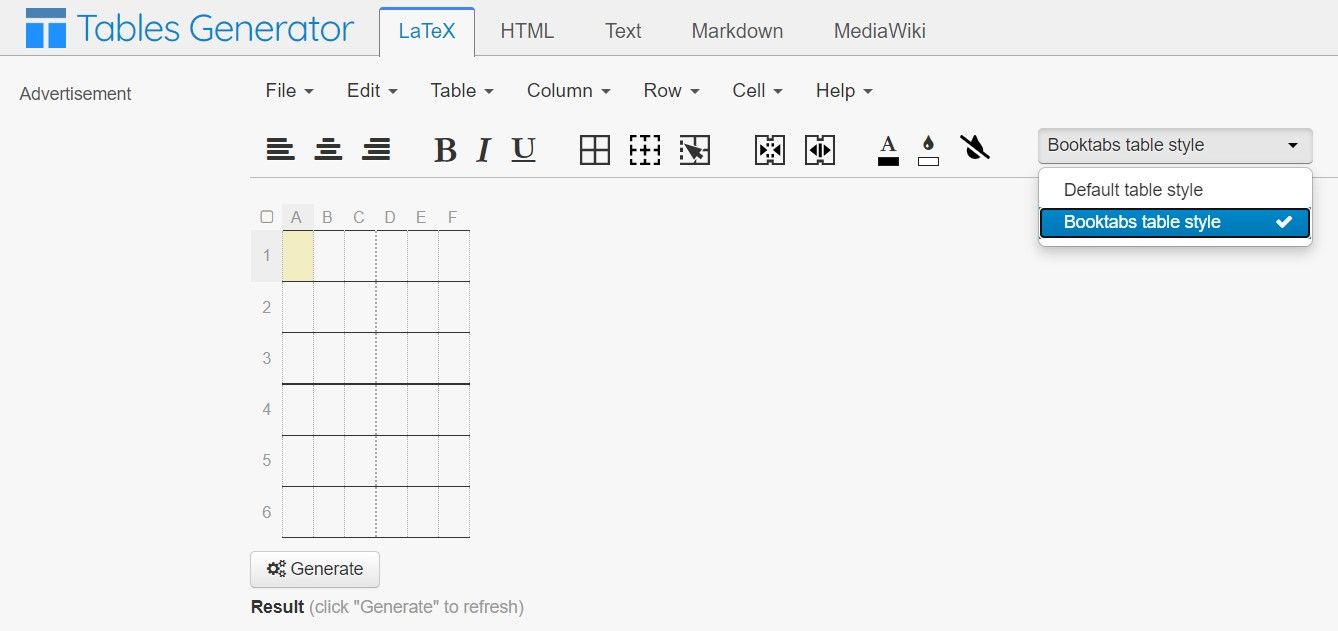
\includegraphics[width=14cm, fbox]{Figures/tablesgenerator.jpg}
\caption{Create a Booktabs style table}
\label{fig:tablegenerator} 
\end{figure}

Use  \texttt{$\backslash$enquote} for double-quotes. \enquote{This is a sample quote.}

Also can try to refer to this image in \autoref{fig:boundingboxexample}. Notice that the \texttt{.eps} and \texttt{.pdf} format vector graphs are favoured, because:

\begin{enumerate}
    \item they can be zoomed-in to check the detail.
    \item text in such formats are search-able.
\end{enumerate}


\begin{figure}[ht]
\centering
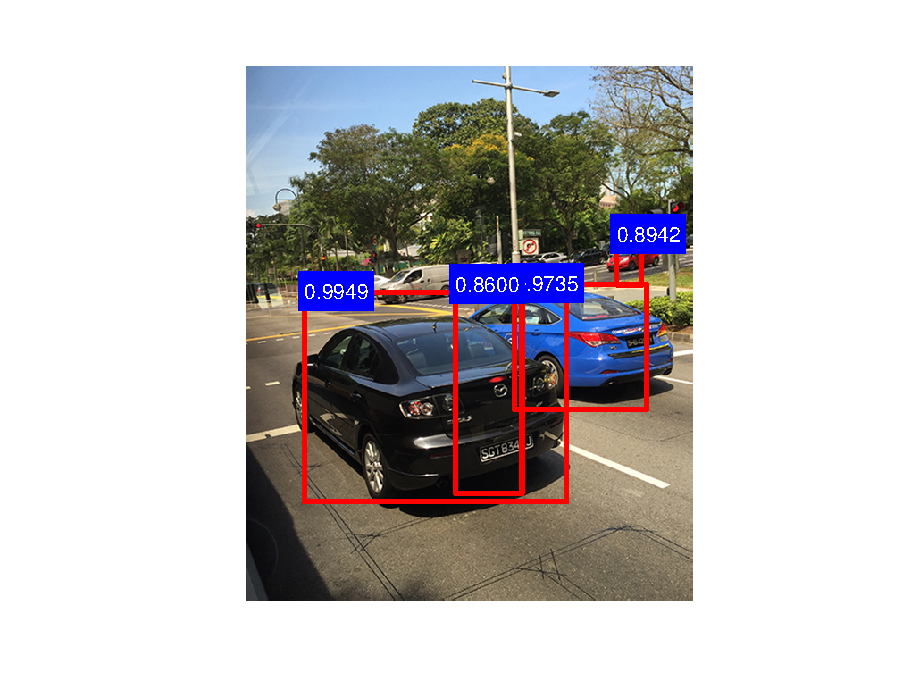
\includegraphics[width=4in, fbox]{Figures/boundingbox.eps}
\caption{Bounding-box example of cars.}
\label{fig:boundingboxexample} 
\end{figure}

Try to insert a math equation as in \autoref{eq:euler}. If you wanna try the in-line mathematical, here is a sample $\alpha = \pi \cdot \frac{1}{\Theta}$.

\begin{equation}
\label{eq:euler}
    e^{ix}= \cos{x} + i \sin{x}
\end{equation}

%Also here is a sample for footnote and hyperlink url\footnote{\url{https://github.com/doem97}}. 

When mention some file formats can use \texttt{music.mp3}, \texttt{latex.pdf}, etc.




\section{Sub-chapter Two}

Contrary to popular belief, Lorem Ipsum is not simply random text. It has roots in a piece of 
\todo{This is a todo note which appears in the margin}
classical Latin literature from 45 BC, making it over 2000 years old. Richard McClintock, a Latin professor at Hampden-Sydney College in Virginia, looked up one of the more obscure Latin words, consectetur, from a Lorem Ipsum passage, and going through the cites of the word in classical literature, discovered the undoubtable source. Lorem Ipsum comes from sections 1.10.32 and 1.10.33 of de Finibus Bonorum et Malorum (The Extremes of Good and Evil) by Cicero, written in 45 BC. This book is a treatise on the theory of ethics, very popular during the Renaissance. The first line of Lorem Ipsum, \enquote{Lorem ipsum dolor sit amet}.., comes from a line in section 1.10.32.

It is a long established fact that a reader will be distracted by the readable content of a page when looking at its layout. The point of using Lorem Ipsum is that it has a more-or-less normal distribution of letters, as opposed to using 'Content here, content here', making it look like readable English. Many desktop publishing packages and web page editors now use Lorem Ipsum as their default model text, and a search for 'lorem ipsum' will uncover many web sites still in their infancy. Various versions have evolved over the years, sometimes by accident, sometimes on purpose (injected humour and the like).

\section{Sub-chapter Three}
\todo[inline]{This todo note appears in line with the text. Todo notes are a great tool to leave comments or notes for self and can then be simply commented out.}
Vivamus eget odio tellus. Nam libero augue, eleifend molestie est eu, tempus vehicula magna. Sed dignissim imperdiet urna, non viverra risus blandit in. In lacinia aliquet leo, ut interdum ipsum ornare sed. Praesent ac fringilla justo. Vivamus pharetra non ipsum eget semper. In hac habitasse platea dictumst. Donec neque lectus, ultricies id massa posuere, sodales interdum ante. Sed et nunc vitae urna ornare porttitor nec vitae urna. Curabitur sit amet luctus urna. Nulla porta malesuada rutrum. Pellentesque vitae velit sed odio tincidunt iaculis. Nulla facilisi.

\newpage

\section{Sub-chapter Four}

To create a bulleted list you need to make use of the ''itemize" environment. A \LaTeX environment is a special section within a page where items as placed. An environment always has a ``\textbackslash{begin}" and a ``\textbackslash{end}". Items you can place in such an environment include:
\begin{itemize}
    \item enumerate -- used to create numbered/letter lists
    \item itemize -- creates a bullet list
    \item figures -- to add images or figures (.eps is the recommended format
    \item tables -- you can create them in tablesgenerator.com then copy the \LaTeX\\code and paste it.
    \item equations -- for those really neat looking mathematical formulae
    \item this list is not exhaustive...
\end{itemize}

\newpage
\section{Sub-chapter Five}
The following are some of the most common commands used during your writing. Some characters are reserved and cannot be directly written as in a normal word processor but need to be ``escaped". Then there are other useful commands such as adding a footnote, inserting a new line (to begin a new paragraph after a blank line, adding labels to items for cross-referencing, etc.

\begin{itemize}
    \item The following are special characters which require a \textbackslash{} before each character so the character is reproduced on the output. The tilde and exponent are even more special. 
    \begin{itemize}
        \item \textbackslash{\#}
        \item \textbackslash{\$}
        \item \textbackslash{\%} -- comment
        \item \textbackslash{\&}
        \item \textbackslash{\_}
        \item \textasciitilde -- type \textbackslash{textasciitilde}
        \item \textasciicircum -- type \textbackslash{textasciicircum}
    \end{itemize}
    \item \textbackslash{textbf} -- bold font
    \item \textbackslash{textit} -- italics
    \item \textbackslash{underline\{words to underline\}}
    \item \textbackslash{emph} -- emphasized text. If used within an italicized text, the output is normal font. If used by itself, text in its argument is italicized.
\end{itemize}
An example highlighting the use of \textbackslash{emph}.
\begin{itemize}
    \item An example of emphasized text with \emph{these words emphasized} within normal font.
    \item \textit{This is an example where \emph{these three words} are emphasized within italicized font}
\end{itemize}

\end{spacing}
%=== END OF CHAPTER ONE ===
\newpage



%=== CHAPTER TWO (2) ===
%=== Literature Review ===

% TODO: Add the .bib references so that they are listed properly.

\chapter{Literature Review}
\begin{spacing}{2.0}
	%\setlength{\parskip}{0.2in}

	\section{Chapter Introduction}

	Video games are constantly evolving to provide more engaging and immersive experiences to players, be it by improved graphics fidelity, better story telling, or by increasing the challenge.
	When it comes to the balancing difficulty to player skill, traditional difficulty techniques often fail to properly adapt to the vast range of player skill levels, and the difference on how fast certain players learn.
	Dynamic Difficulty Adjustment (DDA), along with Reinforcement Learning (RL) agents emerge as solutions to adapt game difficulty in real time based on player performance, along with decreasing predictability and
	increasing the challenge players face, enhancing player immersion, motivation and increasing replayability \cite{grech_creating_2023} \cite{mercieca_evaluating_2023} \cite{attard_analysing_2021}. This section explores and discusses previous works and their results regarding DDA and RL agents in video games
	to identify the current state of the art and to provide a foundation for the research conducted in this thesis.

	% make dda come after Unity-ML.
	\section{Dynamic Difficulty Adjustment (DDA)}

	Dynamic Difficulty Adjustment (DDA) refers to a game design approach where a set of systems dynamically alter the difficulty of a game through modifying game parameters such as AI behaviour,
	player and enemy stats, or environmental factors in real time to match player's skill. These systems target maintaining player engagement to be in line with Csikszentmihalyi's Flow Model, also known as the
	"flow state", a mental condition that is characterised by its ability to keep players deeply immersed and focus on gameplay, avoiding boredom or frustration \cite{grech_creating_2023} \cite{mifsud_utilizing_2021} \cite{laus_dynamic_2022} \cite{vang_impact_2022}.

	% Mention the flow state a bit more
	\begin{figure}[ht]
		\centering
		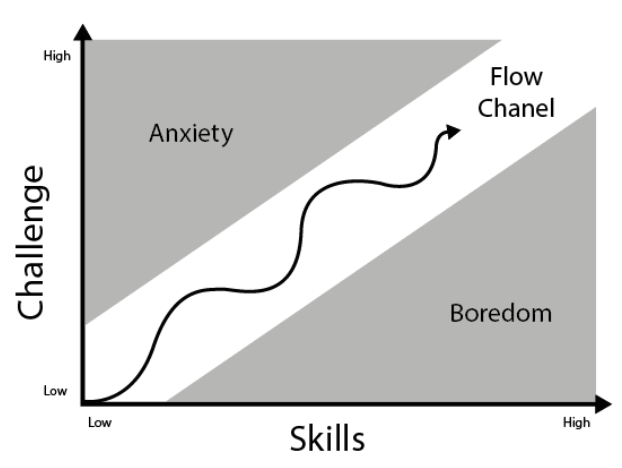
\includegraphics[width=5in, fbox]{Figures/Flow_State.png}
		\caption{Flow State. \cite{sepulveda_exploring_2019}}
		\label{fig:flowstate}
	\end{figure}

	One of the fundamental aspects of DDA is its adaptability to player performance, which allows it to better accomodate the diverse range of player skill levels and learning speeds, avoiding the frustration that
	can occur with traditional fixed difficulty settings. Research has shown that several DDA implementations, such as ramping (rDDA) and player-controlled adjustments (pDDA), can significantly improve player experience.
	And recently, these approaches on DDA have been combined with AI techniques and algorithms to create more sophisticated and responsive systems that can adapt to player performance in real time, such as
	Deep Reinforcement Learning (DRL), Fuzzy Logic, Decision trees and Monte Carlo Tree Search (MCTS) \cite{attard_analysing_2021} \cite{chrysafiadi_fuzzy_based_2023}.
	% Mention the specific data needed for DDA to work in these types of games \cite{grech_creating_2023}

	\subsection{Determining Player Skill}

	Determining player skill is a crucial aspect of DDA, as if the DDA system is innaccurate, it can lead to the opposite effect, where the player will become more bored or frustrated, and can even lead to player's
	leaving the game. To develop effective DDA systems, it is crucial that developers take care to choose the variables that best determine the player's skill level. In the work done by Hunicke {31}, the Hamlet DDA system was used to
	closely monitor the core inventory, including the players health, shielding, ammunition, and weapons, adjusting the difficulty of the level based on the player's items. In a combat encounter, the DDA system was
	developed to see rapid depletion of items as a sign of player struggle, and therefore the system would intervene by modifying the level to aid the player {31}.

	\section{Static Game Difficulties}

	Currently, most games use static difficulty settings, where players choose a static difficulty level before starting the game.
	There are many reasons for this, such as the simplicity of implementation, the ability to control the player experience
	and progression, and that in the past players did not like the instability of dynamic difficulty systems, which with older algorithms
	did not have access nor the ability to process the complex data needed for DDA to work in these types of games \cite{attard_analysing_2021}

	\subsection{Fixed Difficulties}

	These fixed difficulties rely on pre-set levels (e.g., easy, medium, hard) chosen by players before playing, and suffer from
	being rigid and unable to adapt to player performance, skill levels or evolving gameplay dynamics \cite{attard_analysing_2021} \cite{laus_dynamic_2022}.
	% Discuss more

	\subsection{Difficulty Selection}

	With difficulty selection, players can change the difficulty during gameplay, helping in reducing the frustration or boredom that
	comes from fixed difficulties, and helps in keeping players engaged for longer periods \cite{attard_analysing_2021} \cite{laus_dynamic_2022}. However, this approach still requires players to manually adjust the difficulty,
	which can be cumbersome and disrupt the flow of the game, and are still rigid in nature, leading to the difficulty always being either too easy or too hard \cite{attard_analysing_2021} \cite{laus_dynamic_2022}.
	% Discuss more

	\section{Dynamic Difficulty Adjustment Compared with Static Difficulties}

	As discussed, dynamic systems outperform static ones when it comes to keeping to Csikszentmihalyi's Flow Model, helping reduce player boredom and frustration while enhancing both player immersion and replayability,
	thus keeping players engaged for longer periods \cite{grech_creating_2023} \cite{attard_analysing_2021} \cite{mifsud_utilizing_2021}. The main drawbacks of DDA come from its more complex development process, the need for more data and computational resources, and the potential for it to
	become more boring and frustrating than fixed difficulties if not implemented correctly, and given an adequate amount of real-time data \cite{attard_analysing_2021} \cite{laus_dynamic_2022}.

	\subsection{Game Immersion and replayability}

	Studies such as those done by \cite{mercieca_evaluating_2023} \cite{attard_analysing_2021} \cite{mifsud_utilizing_2021} \cite{laus_dynamic_2022} \cite{vang_impact_2022} confirm that DDA significantly improves player immersion by keeping players in a balanced challenge zone, keeping them both motivated and better entertained, resulting in
	a better player experience. Furthermore, the dynamic nature of these systems motivate players to revisit games, as the change in difficulty and challenges they present the player scale with the player's skill,
	keeping the game feeling fresh and engaging where fixed difficulties could not \cite{grech_creating_2023} \cite{attard_analysing_2021} \cite{mifsud_utilizing_2021} \cite{laus_dynamic_2022} \cite{sepulveda_exploring_2019}.

	\section{AI with DDA Algorithms}

	Studies have also shown that in recent time, AI has played a pivotal role in improving on the implementation of DDA systems by allowing better decision making and data processing based on player performance metrics.
	Such models are Reinforcement Learning (RL), as shown in the work done by \cite{mercieca_evaluating_2023} \cite{mifsud_utilizing_2021} \cite{zheng_dynamic_2024}, fuzzy logic \cite{chrysafiadi_fuzzy_based_2023}, Monte Carlo Tree Search (MCTS) \cite{demediuk_monte_2017} \cite{soemers_enhancements_2016}, and Decision Trees \cite{sejrsgaard_jacobsen_dynamic_2011}, also known as Behaviour trees.
	These different AI algorithms have helped enable more nuanced and responsive DDA implementations, offering players what feels like a more tailored experience \cite{attard_analysing_2021} \cite{vodopivec_monte_2017} \cite{chrysafiadi_fuzzy_based_2023}.

	\section{Adaptive Gameplay AI Algorithms}

	\subsection{Deep Reinforcement Learning (DRL) Algorithm}

	% TODO: Go more in depths about PPO, since it is the most common algorithm used in games.
	RL algorithms, and in turn Deep Reinforcement Learning (DRL) algorithms use neural networks to enable AI agents to learn and adapt to the situation presented to them. This is done through multiple methods, with the
	most common being Proximal Policy Optimisation (PPO), the State Action Reward State Action (SARSA) and Q-learning algorithms, which have been used to great effect in games like \cite{bin_ramlan_implementation_2021} \cite{metz_evaluation_2020}. They work by placing the agent in a controlled environment,
	where they learn through trial and error, being rewarded for good decisions and penalised for poor ones. This causes the agent to learn the optimal strategy for the situation presented to them,
	and can be used not only as opponents or allies in games, but also as a way to dynamically adjust game difficulty in real time, particularly in fighting games and other high-interaction environments,
	as seen in the works done by \cite{mercieca_evaluating_2023} \cite{mifsud_utilizing_2021} \cite{zheng_dynamic_2024}.
	% Discuss these works a lot more in the RL Agents section, which will be moved above this.

	% Mention the flow state a bit more
	\begin{figure}[ht]
		\centering
		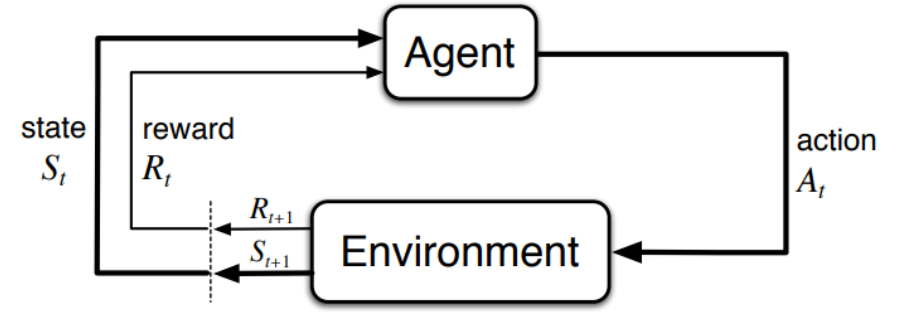
\includegraphics[width=5in, fbox]{Figures/SarSa.png}
		\caption{Agent training environment interaction in RL. \cite{grech_creating_2023}}
		\label{fig:rl_training}
	\end{figure}

	% Should likely expand, but only once the latter part about RL-Agents is done. On top of that, too much time has been spent fine tuning this, and as such it is likely better to move on to the other sections and then come back to it.
	% Q-Learning and Proximal Policy Optimisation (PPO) algorithms, which have been used to
	% Algorithms such as Proximal Policy Optimization (PPO) have been effective in tailoring game difficulty in real time, particularly in fighting games and other high-interaction environments \cite{bin_ramlan_implementation_2021} \cite{metz_evaluation_2020}.

	\subsection{Fuzzy Logic}

	In the study done by Chrysafiadi, et al. \cite{chrysafiadi_fuzzy_based_2023}, Fuzzy logic systems were employed to dynamically adjust game difficulty to match the player's skill level, with the goal of maintaining player engagement while teaching them HTML programming.
	Fuzzy logic systems are particularly effective in such real-time adjustments, as they require less training data when compared to ML models. Moreover, trhese systems offer immediate real-time adjustments to better align with player performance.
	The results of this study show that player dropouts decreased significantly, and player engagement and motivation increased, and even performed better than other groups, proving that fuzzy-based DDA can enhance
	educational outcomes and help keep players in the Flow State with reduced data \cite{chrysafiadi_fuzzy_based_2023}.
	% Perhaps add statistics and more information on the study?

	\subsection{Monte Carlo Tree Search (MCTS)}

	MCTS works by exploring different game states in the form of simulations to optimise decision-making, and is done by building a search tree iteratively, balancing exploration and exploitation to find the best
	move \cite{vodopivec_monte_2017} \cite{demediuk_monte_2017}. In the work done by Demediuk, et al. \cite{demediuk_monte_2017}, MCTS was used to enhance player engagement by modifying AI strategies to maintain balanced matches, with variants like Reactive Outcome-Sensitive Action Selection (ROSAS).
	ROSAS is reactive in nature, which can make it feel unnatural, whilst Proactive OSAS (POSAS), which is more proactive and can feel more natural, at the cost of precision. In the work done by Soemers, et al. \cite{soemers_enhancements_2016},
	different MCTS optimisations were made, such as Progressive History (PH) and N-Gram Selection Technique (NST), where PH biases the selection step towards actions that have been successful in the past, and NST
	biases the play-out step towards actions that have been successful in the past, with the results showing that when combined these greatly improve the algorithm's performance. Another improvement was Deteministic
	Game Detection (DGD), which modifies MCTS behaviour to optimise for deterministic games by using alternative evaluation strategies, which was effective when combined with other enhancements \cite{soemers_enhancements_2016}.
	What these studies show, is that when it comes to more complex and deterministic games, MCTS can be a powerful tool to enhance player engagement both as an opponent, as well as a tool to dynamically adjust
	game difficulty.

	\subsection{Decision \& Behaviour Trees}

	% TODO: Split Decision and behaviour trees based on extra research done.
	Decision trees are popular tools in data analysis, and are used for classification and prediction due to their intuitive structure, which include nodes (root, internal, leaf) and branches \cite{song_decision_2015} \cite{mienye_survey_2024}.
	The framework around how decision trees work when it comes to games varies, as not only can it reduce code repetition in game development, both for complex and simple games \cite{vuong_artificial_2020}, but its structure allows for easy
	interpretation and visualisation of the algorithm's decision making process, making them particularly useful for adapting game features dynamically, as seen in the work done by \cite{sejrsgaard_jacobsen_dynamic_2011}.
	Their approach involved examining two distinct approaches, one using predefined behaviour trees of varying difficulties, and another employing a single tree with dynamic adjustment of probabilities to alter difficulty.
	The first approach struggled when it came to flexibility, as it could not adapt to player performance, which was in stark contrast with the second approach, which was able to optimise behaviour probabilities
	and display superior adaptability, helping to keep the player in the Flow State, and maintain player engagement \cite{sejrsgaard_jacobsen_dynamic_2011}. Along with this, decision trees have been shown to be even more effective when combined with
	other algorithms, such as RL, which help greatly in improving their efficiency and scalability in complex gaming environments, or even with state machines in more simple environments \cite{mcquillan_survey_nodate} \cite{sejrsgaard_jacobsen_dynamic_2011}.

	% Here

	\section{Procedural Content Generation}

	Procedural Content Generation (PCG) is a technique used in game development to create game content algorithmically, leveraging algorithms to dynamically create and add content such as levels, environments,
	and items to games that both help in reducing development time and costs, but also increase replayability and can easily be combined with DDA systems to create more engaging and immersive experiences \cite{laus_dynamic_2022}.
	When paired not only with DDA, but also with AI agents, such as those created by \cite{grech_creating_2023}, PCG was used to constantly modify the best possible action that the player and the agent could take, which in turn
	not only forced the player to adapt to the changing environent, but also helped keep the player feeling challenged and engaged, avoiding frustration since the opponent was also having to adapt in a human like way,
	helping in keeping the player in the Flow State.
	% This needs to be cut down and made better

	% Should finite state machines be included here?

	\section{Unity ML-Agents and how they work}

	Unity ML Agents is a toolkit that enables developers to more easily create and integrate intelligent agents within Unity environments using Machine Learning (ML) techniques.
	The package allows users to transform any scene into a training enviroment where agents can be trained using algorithms such as RL, Imitation Learning and neuroevolution, by allowing agents to observe their surroundings, take actions and receive rewards,
	as well as specifying the behaviours that these agents can take \cite{raut_unity_2024} \cite{unity_ml_agents}.

	\subsection{Finite State Machines}

	Traditionally, and even to this day the most common way to implement AI in games is through Finite State Machines (FSM), which are used to describe a relationship between a set of states, where transitions
	between these states are determined by condition, with actions being performed based on the current state \cite{grech_creating_2023}. FSMs are useful in simple environments, however as the number of actions and states are limited, However
	as the number of states increase, so does the complexity of the FSM, making it difficult to manage, debug and maintain \cite{grech_creating_2023}.

	\subsection{RL Agents}

	As mentioned in an earlier section, RL agents are AI agents that learn through trial and error, being rewarded for good decisions and penalised for poor ones. RL-Agents trained using Unity ML-Agents have more
	access to the environment and its data, and this has been used in the work done by Grech \cite{grech_creating_2023}, where he trained an RL-Agent to act as an opponent in a Real Time Strategy (RTS) game, taking multiple stages of the agent
	in training for the different difficulties. There were also different RL-Agent models such as the Proximal Policy Optimisation (PPO) and others that were used to act as enemies in fighting games \cite{bin_ramlan_implementation_2021}, bosses \cite{metz_evaluation_2020},
	and even for racing games \cite{berta_development_2024}. In these works, along with those done by \cite{borg_investigating_2020} \cite{zhasulanov_enhancing_2024} \cite{raut_unity_2024}, it was revealed that RL-Agents have shown many times to be an effective way to make a more unpredictable, life-like and challenging
	opponent for player, significantly boosting their experience and engagement.

	\subsection{RL Agents compared with Finite State Machines}

	The main differences between FSMs and RL-Agents are their development time and costs, as FSM's are easier and cheaper to implement, but are then limited in their complexity and scalability, where as RL-Agents
	take more time and resources to develop, but solve the issues with FSMs being their complexity, scalability, and the simple fact that when a player fights an FSM enough, they will learn the patterns and states,
	making the game predictable and boring \cite{grech_creating_2023} \cite{bin_ramlan_implementation_2021} \cite{metz_evaluation_2020}. This life-like aspect to RL-Agents can, and have been shown to greatly improve game replayability and immersion, keeping the player in the flow state for longer
	and providing a superior experience to the player \cite{grech_creating_2023} \cite{bin_ramlan_implementation_2021} \cite{metz_evaluation_2020}. With all of this however, it is important to not that if an RL-Agent is not implemented or trained correctly, it can lead to the opposite effect,
	where an opponent is too difficult, leading to player frustration, or too easy, leading to player boredom \cite{grech_creating_2023} \cite{bin_ramlan_implementation_2021} \cite{metz_evaluation_2020}.

	\subsection{Practical Applications}

	As mentioned in the previous sections, RL-Agents have been used in a variety of games, from RTS games to fighting games and now even racing games. The practical applications of RL-Agents in games are vast,
	and as hardware capabilities improve, and our understanding and training techniques improve, the potential for RL-Agents in games is almost limitless. The ability to create more engaging, immersive and challenging
	opponents for players, as well as allies, and the ability to easily integrate them with DDA systems, PCG and other game development techniques to make games more replayable and engaging is a powerful tool for developers
	to create better games \cite{grech_creating_2023} \cite{borg_investigating_2020} \cite{zhasulanov_enhancing_2024} \cite{raut_unity_2024} \cite{metz_evaluation_2020}

	\section{Chapter Overview}

	This chapter has provided an overview on the current state of the art in Dynamic Difficulty Adjustment (DDA) and Reinforcement Learning (RL) agents in video games, and how individually they have been used to
	improve upon more static techniques, such as fixed difficulties and Finite State Machines (FSMs). It has shown that integrating AI techniques has helped in improving the accuracy and adaptability of DDA systems,
	and the latest advancements in RL-Agents, including the Unity ML-Agents package, have shown just how revolutionary these techniques are at improving player engagement and immersion, as well as game replayability
	when these techniques are implemented.
	% Should more sources be referenced since this is more of a summary of the chapter?

	% TODO: Some parts have not been added to this from the word document, and some information is currently missing, however too much time has been spent on this draft so it is best to move on to the next section
	% and wait for feedback and then come back to this section to make the necessary changes.
	% On top of that, due to there being too much information not being condensed properly, the analysis is not as deep as it should be, and this should be improved in the next draft following recommendations.

	%=== END OF CHAPTER TWO ===
\end{spacing}
\newpage

%=== CHAPTER THREE (3) ===
%=== (Actual work done and contribution, including literature survey) ===

\chapter{Research Methodology}
\begin{spacing}{2.0}
	%\setlength{\parskip}{0.2in}
	%  (Actual work done and contribution, including literature survey)


	\section{Chapter Introduction}

	% Mention the aim of the study and reference the research questions, using the SOI.

	% Create mini summary of selected research papers and notes to better align the research questions and methodology with the literature review.

	% \section{Nature of Research}
	% % Should I discuss this in its own section, or just include my own notes and split it in the introduction and especiialy discuss it % in the data collection,
	% % as it is more relevant to the data collection and evaluation sections and is covered more in depth there.
	%    \subsection{}

	% Should this just be called the Research Pipeline?
	\section{Conceptual Framework}

	Figure \ref{fig:pipeline} outlines the methodology pipeline for this study's research, with it being divided into 4 major sections.
	The first section consisted of decided on the prerequisites and tools required for the development of the prototype, along with developing the
	traditional game mechanics and State Machine opponent. The second section consisted of setting up the training scene and Unity mL-Agents plugin,
	training, and evaluating the RL-Agent. The third section involved developing the data collection and developing the DDA system using behaviour-trees,
	which were decided over the other options due to their ease-of-use, and how well they are at representing the AI's decision making process.
	Finally, the prototype was evaluated by the participants, with the data collected being analysed and compared to previous research to answer the research questions.

	\begin{figure}[ht]
		\centering
		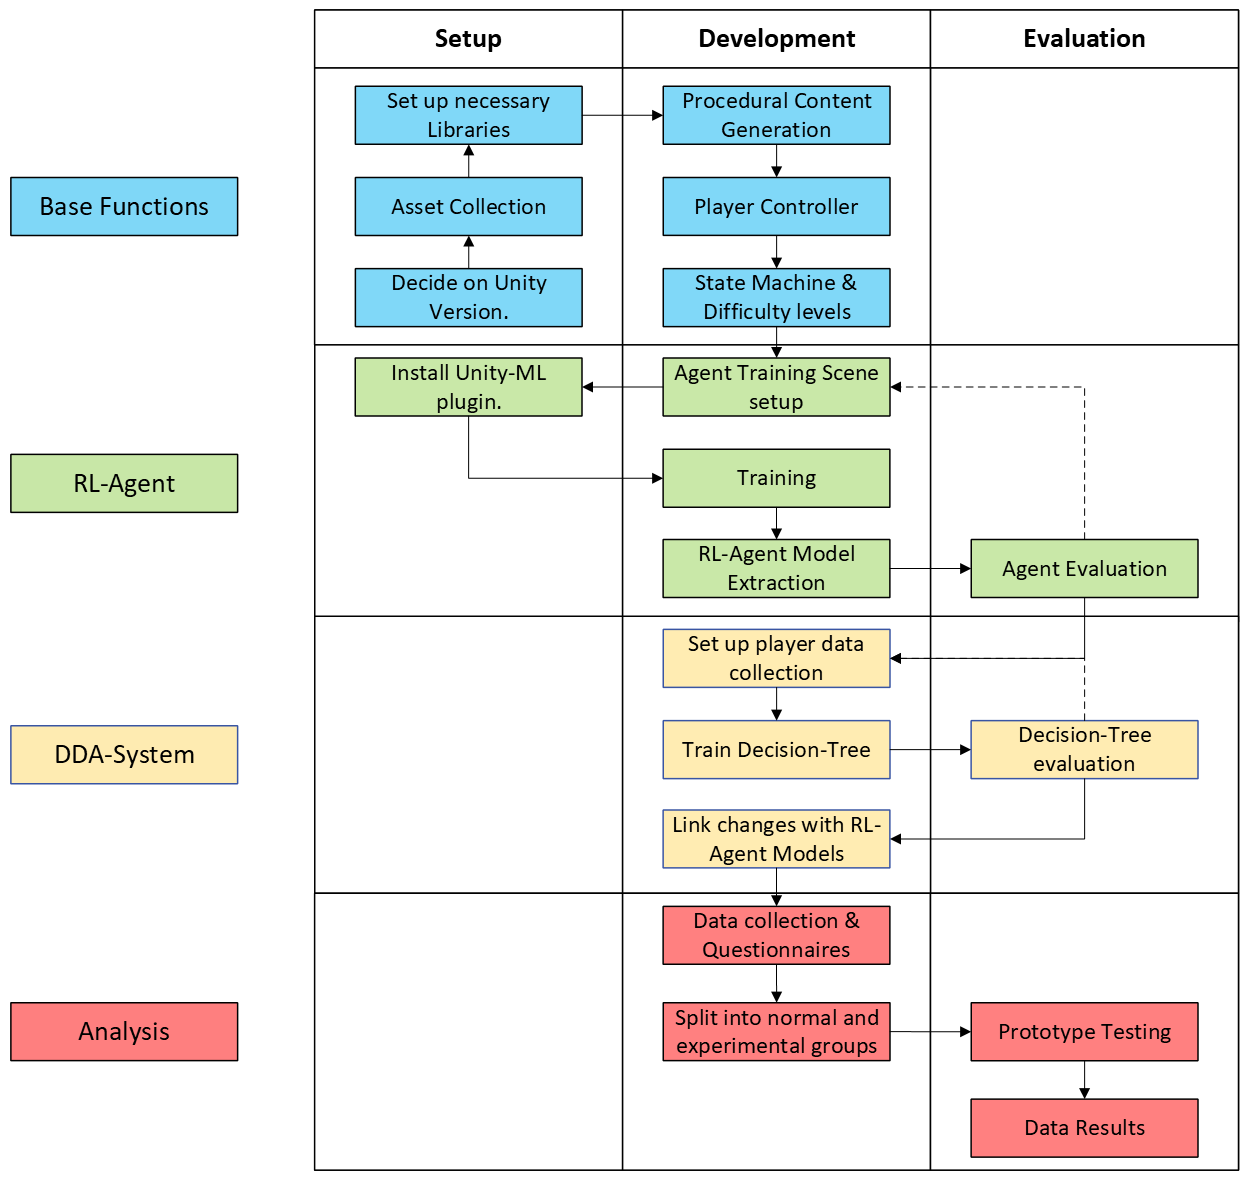
\includegraphics[width=5in, fbox]{Figures/ResearchPipeline.png}
		\caption{Diagram representing the methodology pipeline.}
		\label{fig:pipeline}
	\end{figure}

	\section{Prerequisites and Tools}

	Before starting development on the prototype, a github repository for the project was created, and Jetbrains Rider was used as the IDE for the project.
	The prototype was developed using Unity 6000.0.31f1, and utilised several Unity packages, assets and plugins, which are listed below:

	% Do I list them here or reference an appendix?

	Along with the built-in Unity packages, the project also used the Unity ML-Agents package which was cloned off the Unity ML-Agents github repository, and the Unity ML-Agents Toolkit, which was cloned off the Unity ML-Agents Toolkit github repository,
	and then imported into the project as a Unity package along with the ML-Agents Extensions packages. The version of ML-Agents used in the prototype
	was version 22, the latest version at the time of development.

	\section{Prototype Outline \& Implementation}

	% Likely will need to split this into an outline, with the State Machine being a subsection, and the RL-Agent and DDA system being their own sections.

	A Prototype game was developed to implement and test the RL-Agent and DDA system for their effectiveness in creating a dynamic and adaptive game experience.
	The core gameplay will consists of traversing the game world in a third person perspective, with the goal to mine and deposit as many ores as possible.
	There are 3 main mechanics which for the core gameplay loop of the game, the scoring system, the mining system, and the inventory system. The mining system is responsible for the player's ability to mine ores,
	the scoring system is responsible for tracking the player's score and awarding them points based on the types or ores deposited, and the inventory system is responsible for forcing the player to carefully
	think about their inventory space and which ores to mine and when to go deposit. The ores and terrain are procedurally generated, with some small obstacles which can force the player to take a slightly longer path.

	\begin{figure}[ht]
		\centering
		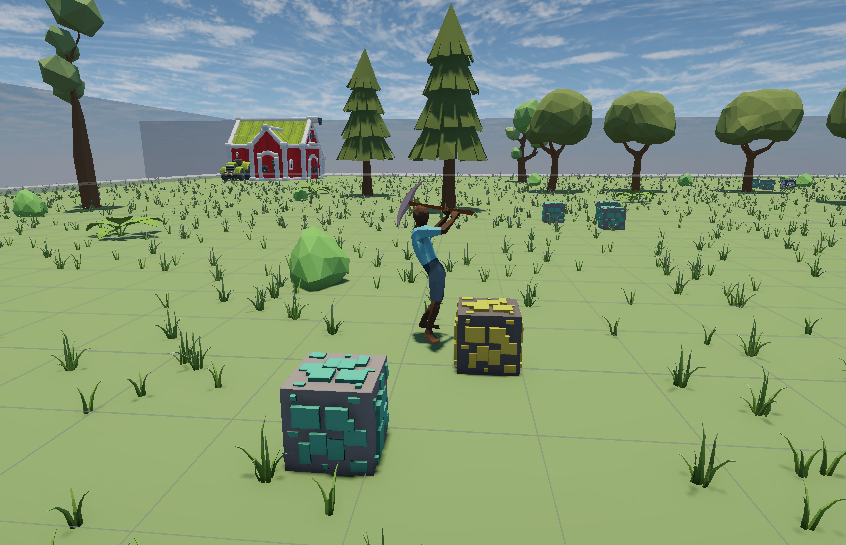
\includegraphics[width=5in, fbox]{Figures/Gameplay.png}
		\caption{Screenshot of gameplay showing the gathering of resouces.}
		\label{fig:gameplay}
	\end{figure}

	The main challenge the player will face is the AI opponent which has the same goal and capabilities of the player. The objective for both of them is to gather as many points as possible before the game ends.
	If the player has more points at the end, they win, if its the same, it is a draw, and if the AI has more points, the player loses. The AI opponent will be different for each stage of the test, with the first
	being a State Machine, and the second being an RL-Agent. More information regarding the test stages and how data will be gathered and analysed will be discussed in a later section.

	\subsection{Ores}

	There are three types of ores in the game, Copper, Silver, and Gold. Each ore is visually distinct, as can be seen in Figure \ref{ores} and have a different chance of spawning, as listed in Table \ref{ore_chance_table}.

	\begin{figure}[ht]
		\centering
		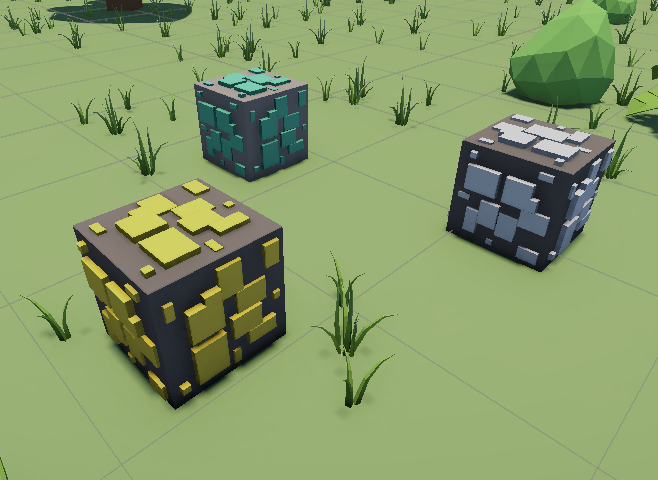
\includegraphics[width=5in, fbox]{Figures/Ores.png}
		\caption{Screenshot showing the different ores.}
		\label{fig:ores}
	\end{figure}

	\begin{table}[ht]
		\centering
		\renewcommand{\arraystretch}{1.2} % Adjust row spacing
		\setlength{\tabcolsep}{8pt} % Adjust column spacing
		\begin{tabular}{|c|c|c|c|}
			\hline
			\textbf{Difficulty} & \textbf{Copper Spawn \%} & \textbf{Silver Spawn \%} & \textbf{Gold Spawn \%} \\
			\hline
			Easy                & 60\%                     & 30\%                     & 10\%                   \\
			\hline
			Medium              & 70\%                     & 25\%                     & 5\%                    \\
			\hline
			Hard                & 75\%                     & 20\%                     & 5\%                    \\
			\hline
		\end{tabular}
		\caption{Chance of spawning for each ore.}
		\label{ore_chance_table}
	\end{table}

	They also take different amounts of time to mine, inventory space, and points awarded when deposited, as listed in Table \ref{ore_table}.

	\begin{table}[ht]
		\centering
		\renewcommand{\arraystretch}{1.2} % Adjust row spacing
		\setlength{\tabcolsep}{8pt} % Adjust column spacing
		\begin{tabular}{|c|c|c|c|}
			\hline
			\textbf{Resource Type} & \textbf{Score} & \textbf{Mining Time (swings)} & \textbf{Inventory Space Taken} \\
			\hline
			Copper                 & 2              & 3                             & 1                              \\
			\hline
			Silver                 & 5              & 5                             & 3                              \\
			\hline
			Gold                   & 10             & 8                             & 5                              \\
			\hline
		\end{tabular}
		\caption{Ore statistics.}
		\label{ore_table}
	\end{table}

	\subsection{Traditional State Machine}

	The State Machince will be a simple AI opponent using the Unity navmesh system to navigate the game world. The AI will have 3 states, a mining state, a depositing state, and a travelling state.
	After completing a task, the AI will use a Physics OverlapSphere to search for the best ore within the vicinity, and once the best option is found, the AI will navigate to the ore and mine it.
	The speed at which the AI travels, and the radius it searches for ores will be adjusted based on the difficulty selected, allowing for a faster and more effective opponent on higher difficulties.
	Once the inventory is full, the AI will navigate to the closest deposit point to deposit the ore and gain points.

	\subsection{RL Agent}

	The Reinforcment Learning Agent will be trained using the Unity ML-Agents plugin, and will use Proximal Policy Optimisation (PPO) as the training algorithm, since it is the most commonly used algorithm due to
	its effectiveness at training agents in complex and continuously changing environments, the main RL training algorithm for the Unity ML-Agents framework, and the one used in the works done by \cite{grech_creating_2023},
    \cite{bin_ramlan_implementation_2021}, \cite{berta_development_2024}, and \cite{raut_unity_2024}.
	The agent will then be placed instead of the State-Machine as the opponent the player will face. More information on the training and evaluation will be discussed in a later section.

	\subsection{DDA System}

	This section will be created over time while the prototype and DDA system are being developed and tested.

	\section{RL-Agent opponent}

	\subsection{Agent Observations}

	To understand the game enviroment, the agent is supplied with several variables to observe via the Unity ML-Agents plugin. These variables are all normalised numerical values between 0 and 1, and are as follows:

	\begin{itemize}
		\item The type of ore currently being obesrved.
		\item How much of the inventory the ore will take up.
		\item The agents normalised position from the ore.
		\item The player's normalised position from the ore.
		\item The deposit point's normalised position from the ore.
		\item The normalised amount of inventory space left.
		\item The normalised amount of time left.
	\end{itemize}

	\begin{figure}[ht]
		\centering
		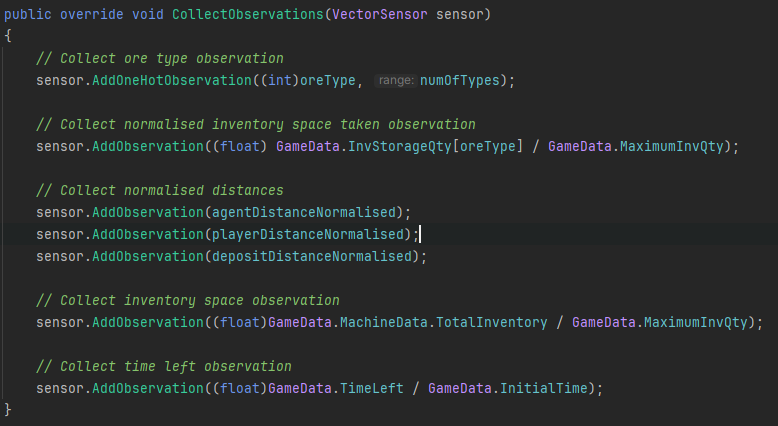
\includegraphics[width=5in, fbox]{Figures/Observations.png}
		\caption{Screenshot showing the Agent's observations.}
		\label{fig:observations}
	\end{figure}

	\subsection{Agent Decisions \& Actions}

	The Agent has 3 decisions it can make, and 2 actions it can take. The decisions are between travelling to and mining the ore being observed, travelling to the deposit point, or observing the next ore.
	The travel to \& mining action involves setting the ore's position as the NavmeshAgent's destination, waiting until the agent arrives, and then mine the ore. Sometimes due to obstacles and the agent's pathfinding,
	the agent may get stuck, which the program will detect very quickly by requesting the agent to decide on another ore. While this is not ideal, it is an uncommon bug with the NavmeshAgent.
	The other action the agent can take is travelling to the deposit point, which acts similarly to the travel to \& mining action, but instead of mining, the agent will just observe and make another decision once it arrives.

	% NOTE: Add flowchart of the agent's decision making process here.

	% TODO: Expand on the agent's observation and decision making.

	\subsection{Agent Rewards \& Penalties}

	A simple reward and penalty system was used to train the agent, since the enviroment is simple and the agent's goal is clear. The focus was on rewarding the agent for mining and depositing ores,
	and penalising them for travelling for too long.

	% TODO: Show the final rewards and penalty systems that will be used

	\subsection{Agent Training}

	\subsection{Model Selection \& Evaluation}

	\section{Data Collection}

	% Should the participants come before the type of data?
	% Should i mention the tests and how the data will be gathered after the sub sections, and use the sub sections to explain the type of data, why it is being collected and who it is being collected from, or should this come before?

	It was decided to use a mixed-methods approach for the evaluation of the prototype, with the majority of the data being quantitative.
	This was chosen to better match \cite{grech_creating_2023} \& \cite{mercieca_evaluating_2023}'s approaches, allowing for an in-depth comparison and analysis of results,
	while allowing for a more detailed understanding of the player's experience and recommendations. Quantitative data will be collected through Unity Analytics, allowing data to be extracted from gameplay sessions,
	as well as close ended questionnaires. Quantitative data will be collected through open ended questions in the questionnaire.

	\subsection{Quantitative Data}

	To better understand the performance of the agent and DDA system against a human player, and to compare the two against State Machines, important statistics throughout the game will be tracked, and saved to a database.
	This data will include the player and enemy action logs, the game summary, and the performance summary.

	\subsubsection{Player and Enemy Action Logs}

	These logs, as seen in \ref{fig:logs} will show all note-worthy actions taken by the player and the enemy, detailing the time, action and any relelvant information, such as the time left and score, and will be shown in chronological order.
	This data will be used to analyse the player's and enemy's behaviour and decision making throughout the game.

	\subsubsection{Game \& Perfomance Summary}

	The game summary will show some of the less note-worthy actions taken by the player and enemy, such as time spent mining and travelling. It will also show the final score and the difficulty selected.
	Due to the DDA system in place, some of the statistics will include logs of difficulty adjustments, and the final difficulty the DDA system selected. The performance summary will be used to capture the
	game's performance by tracking metrics such as frame-rate, CPU Usage and memory usage.

	\subsection{Qualitative Data}

	To better understand the player's experience, as well as some pain points of the game, the questionnaires will have some open ended questions, asking the player to better describe their experience,
	and to provide feedback and any recommendations that they might have. This data will help expand upon the metrics gathered from the quantitative data, and will be used to better answer the research questions.

	\subsection{Participants}

	To really gauge the effectiveness of RL-Agents and DDA systems in creating a dynamic and adaptive experience, a large diverse group of participants will be required.
	% TODO: Add more info about the number of participants and such instead of saying large and diverse.
	By having players of different ages and experience, the data collected will be more varied and allow for a more in-depth analysis of the data. This is inline with the research being conducted, as the goal is to
	identify places where AI is worth implementing, such as more difficult competitive games, or games with a more casual audience.

	\subsection{Tests}
	% Mention that they will agree to the notice found at the end of the SOI
	The tests will be conducted in two stages. First, a close-ended questionnaire will be taken by the participants to gather basic information anonymously, such as age and gaming experience. Once complete,
	the participants will be split into two groups, ensuring that both groups have a similar distribution of age and experience, and they will both play the traditional segment of the prototype,
	with traditional difficulty settings and a State Machine as the opponent. In the second stage, the first group will then play against the RL-Agent, whereas the second group will play against the RL-Agent
	with the DDA system in place. After each playtest, the participants will be given a questionnaire to describe their experience and provide feedback, with both closed and open-ended questions. As mentioned earlier,
	data from the playtests will also be gathered through Unity Analytics.

	\section{Evaluation}

	The data collected from the playtests and questionnaires will be analysed and cross-referenced to find any patterns or correlations between the data.
	The quantitative parts of the data will be analysed using T-Test analysis, and the qualitative data will be analysed using thematic analysis. The results will then be compared to previous research,
	and then be used to answer the research questions, and to prove or disprove the hypothesis.

	\section{Chapter Overview}

	%=== END OF CHAPTER THREE ===
\end{spacing}
\newpage

%=== CHAPTER FOUR (4) ===
%=== Test and Experiments ===

\chapter{Analysis of Results and Discussion}
\begin{spacing}{2.0}
%\setlength{\parskip}{0.1in}

\section{One}
This section includes critical discussion about the Student’s findings and shows how these findings support the original objectives laid out for the dissertation, which may be partially or
fully achieved, or even exceeded. The Student may also include new areas of an investigation prompted by developments in the research dissertation. Above all, it is required to present strong arguments which show how findings may offer a valid contribution to the development of the subject of the selected research area or issues related to it. Percentage amount of words in section: 25 \% of Dissertation

\section{Two}

\section{Three}


%=== END OF CHAPTER FOUR ===
\end{spacing}
\newpage

%=== CHAPTER FIVE (5) ===
%=== Discussion ===

\chapter{Conclusions and Recommendations}
\begin{spacing}{2.0}
%\setlength{\parskip}{0.2in}

\section{One}

In this chapter, the Student has to evaluate the significance of the work done and give recommendations for any further investigations. Percentage amount of words in section: 20 \% of Dissertation.

\section{Two}

\section{Three}


%=== END OF CHAPTER FIVE ===
\end{spacing}
\newpage


%==== ENDING PART ===

\renewcommand\bibname{List of References}
\bibliographystyle{IEEEtran}
\begin{spacing}{2.0}
\titlespacing*{\chapter}{0pt}{-18pt}{41pt}
\bibliography{Ref/References}
\end{spacing}
\newpage

%=== APPENDIX ===

\begin{appendices}
\label{cha:appendices}

\chapter{Introduction of Appendix}
\markboth{Appendix A}{} % For appendix first (affects header)
\begin{spacing}{2.0}

Interview summaries, sample questionnaires, and references should be placed in this section. For easier referencing, figures, tables, graphs, photos, diagrams, etc., should be inserted within
the main text such as the literature review, the experimental process or procedure, the results and discussion chapters. Appendices are usually used to present further details about the results. Appendices may be a compulsory part of a dissertation, but they are not treated as part of the dissertation for purposes
of assessing the dissertation. So any material which is significant to judging the quality of the dissertation or of the project as a whole should be in the main body of the dissertation (main text), and not in appendices.

\end{spacing}

\chapter{Sample Code}
\markboth{Appendix B}{} % For appendix second, etc..
\begin{spacing}{2.0}

You can share your GitHub link. Below shows how to insert highlighted source code from the source file.

\end{spacing}

% include the code
\lstinputlisting{Code/sample.py}

\end{appendices}
%==== END OF ALL ===
\end{document}